%%%%%%%%%%%%%%%%%%%%%%%%%%%%%%%%%%%%%%%%%
% Journal Article
% LaTeX Template
% Version 1.3 (9/9/13)
%
% This template has been downloaded from:
% http://www.LaTeXTemplates.com
%
% Original author:
% Frits Wenneker (http://www.howtotex.com)
%
% License:
% CC BY-NC-SA 3.0 (http://creativecommons.org/licenses/by-nc-sa/3.0/)
%
%%%%%%%%%%%%%%%%%%%%%%%%%%%%%%%%%%%%%%%%%

%----------------------------------------------------------------------------------------
%	PACKAGES AND OTHER DOCUMENT CONFIGURATIONS
%----------------------------------------------------------------------------------------

\documentclass[twoside, 11pr]{article}

\usepackage[utf8]{inputenc} % Use 8-bit encoding that has 256 glyphs



\linespread{1.1} % Line spacing - Palatino needs more space between lines
\usepackage{microtype} % Slightly tweak font spacing for aesthetics

\usepackage[a4paper,top=25mm, bottom=25mm, right=25mm, left=25mm]{geometry} % Document margins
\usepackage{multicol} % Used for the two-column layout of the document
\usepackage[hang, small,labelfont=bf,up,textfont=it,up]{caption} % Custom captions under/above floats in tables or figures
\usepackage{booktabs}% Horizontal rules in tables
\usepackage{float} % Required for tables and figures in the multi-column environment - they need to be placed in specific locations with the [H] (e.g. \begin{table}[H])
\usepackage{hyperref} % For hyperlinks in the PDF
\usepackage{graphicx}
\renewcommand\figurename{Fig.}
\usepackage{subfig}
\usepackage{lettrine} % The lettrine is the first enlarged letter at the beginning of the text
\usepackage{paralist} % Used for the compactitem environment which makes bullet points with less space between them

%\usepackage{abstract} % Allows abstract customization
%\renewcommand{\abstractnamefont}{\normalfont\bfseries} % Set the "Abstract" text to bold
%\renewcommand{\abstracttextfont}{\normalfont\small\itshape} % Set the abstract itself to small italic text

%\usepackage{titlesec} % Allows customization of titles
%\renewcommand\thesection{\Roman{section}} % Roman numerals for the sections
%\renewcommand\thesubsection{\Roman{subsection}} % Roman numerals for subsections
%\titlespacing\section{0pt}{15pt plus 4pt minus 2pt}{10pt plus 4pt minus 2pt} % smaller spacing after section-title
%\titleformat{\section}[block]{\large\scshape\centering}{\thesection.}{1em}{} % Change the look of the section titles
%\titleformat{\subsection}[block]{\large}{\thesubsection.}{1em}{} % Change the look of the section titles
%\titleformat{\subsection}[block]{\normalsize\bfseries}{\thesubsection.}{1em}{}

\usepackage{fancyhdr} % Headers and footers
\pagestyle{fancy} % All pages have headers and footers
\fancyhead{} % Blank out the default header
\fancyfoot{} % Blank out the default footer
\renewcommand{\headrulewidth}{0pt} % remove line in header

\usepackage{listings}

\usepackage[ngerman]{babel}								% Sprache: Deutsch


%\fancyhead[L]{Remote Sensing Laboratories, April 2015 $\bullet$ April 2015} % Custom header text
\fancyhead[C]{\textit{Git-Crash-Tutorial}} % Custom header text
%\fancyhead[R]{April 2015} % Custom header text
\fancyfoot[C]{\thepage} % Custom footer text


% use natbib bibliography style
\usepackage{csquotes}
\usepackage{natbib}

\usepackage{textgreek}
\usepackage{amsmath,amsfonts,amssymb}
\usepackage{array}
\providecommand{\abs}[1]{\lvert#1\rvert}




%----------------------------------------------------------------------------------------
%	TITLE SECTION
%----------------------------------------------------------------------------------------

\title{\vspace{-10mm}\fontsize{15pt}{0pt}\selectfont\textbf{Git-Tutorial}} % Article title
\author{
\textsc{Moritz Bruggisser}\\[-9mm] % Your name with footnote
\vspace{-9mm}
}

\date{August 22, 2017}


%----------------------------------------------------------------------------------------

\begin{document}
\maketitle % Insert title
\thispagestyle{fancy} % All pages have headers and footers

%----------------------------------------------------------------------------------------
%	ABSTRACT
%----------------------------------------------------------------------------------------

%\begin{abstract}


%\end{abstract}

%----------------------------------------------------------------------------------------
%	ARTICLE CONTENTS
%----------------------------------------------------------------------------------------

%\begin{multicols}{2} % Two-column layout throughout the main article text


%----------------------------------------------------------------------------------------
%	Introduction
%
% Hier folgt Problem Formulation
%----------------------------------------------------------------------------------------

\section{Einleitung}

Eine Möglichkeit für Version Control ist Git. Hier zeige ich eine sehr einfaches Beispiel anhand von Github. Da ich aber auch noch nicht viel Ahnung habe von all den Möglichkeiten, die Git bietet, beschränke ich mich hier auf die ganz grundsätzlichen Möglichkeiten, sprich: ich zeige, wie man ein Repo (repository) auf einem Server erzeugt, lokal ein File bearbeitet und sichert (in einem lokalen Repo, d.h. hier dann einfach ein Ordner), und wie man das File im lokalen Repo dann ins Repo auf dem Server pushed. \par
In diesem Tutorial konzentriere ich mich auf ein Vorgehen basierend auf dem Terminal von Linux/Mac, für Windows sollte dies jedoch genau gleich funktionieren. Kann's nur gerade nicht überprüfen. Gewisse IDEs bieten aber auch bereits implementierte, grafische Git-Anbindungen, so (meines Wissens nach) PyCharm oder Atom. Diese Möglichkeiten hab ich aber bisher nicht verwendet.\par
Weiter zeige ich das Vorgehen hier für Github, weil man damit einen Gratisaccount erstellen kann, wenn dieser dann auch öffentlich ist. Github bietet zudem ein GUI, allerdings bietet die Github-Homepage die selben Funktionen auch. \par
Alternativ zu Github kann man Git auch auf einem eigenen Server laufen lassen, wenn man denn einen hat. Die Befehle sollten meines Wissens nach auch hier die selben sein, da Git quasi eine Befehlssprache vorgibt.
\newline
\par
Da ich weiterhin noch keine Erfahrung mit Branches etc. habe (sind meinem Verständnis nach alternative \glqq Zweige\grqq (Branches) in der Versionierung eines Scripts, die dazu dienen, zusätzliche Funktionen in die Funktionalität eines Programms einzubauen, ohne die ursprüngliche Version an den Arsch zu machen, auf die man dann aber später zurückgreifen kann, solle man mit den erweiterten Funktionen zufrieden sein), lass ich das hier mal bleiben. Wichtig ist dann nur, dass wir hier immer auf dem Master-Branch arbeiten.

\subsection{Hilfestellungen zu Git-Befehlen}

Tutorials und Erklärungen zu den git-Befehlen findet man über folgende Terminal-Befehle:

\begin{lstlisting}
man git
git --help
\end{lstlisting}

\section{Workflow}

\subsection{Git konfigurieren}

Wie ich's verstehe, muss man Git (d.h. der Git-Verwaltung auf dem eigenen Rechner) zuerst den Account mitteilen, mit welchem man arbeitet (dazu muss man natürlich zuerst einen Account bei Github erstellen). Die Git-Konfiguration kann über einen Benutzernamen erfolgen:

\begin{lstlisting}
git config --global username
\end{lstlisting}

\noindent
oder aber über die Mailadresse, die für die Anmeldung bei Github verwendet wird:

\begin{lstlisting}
git config --global user.email@email.com
\end{lstlisting}


\subsection{Repository auf Server erstellen}\label{ch:gitRepo}

Nun muss man ein Repository (Repo) in Github erstellen, in welches später die Files übertragen (pushed) werden sollen. Dieses Repo ist somit der Ordner auf einem Server, über den jeweils die Änderungen synchronisiert werden (Kapitel \ref{ch:push}). Alle Projektmitarbeiter haben folglich Zugriff auf dieses Repo. \par
Das Repo erstelle ich immer online (auf der Homepage von Github), weiss nicht, ob dies auch über das Terminal möglich wäre oder über das Github-GUI zum runterladen.

\begin{figure*}[!tbph]
\makebox[\textwidth][c]{\begin{minipage}[c]{\textwidth}
\centering
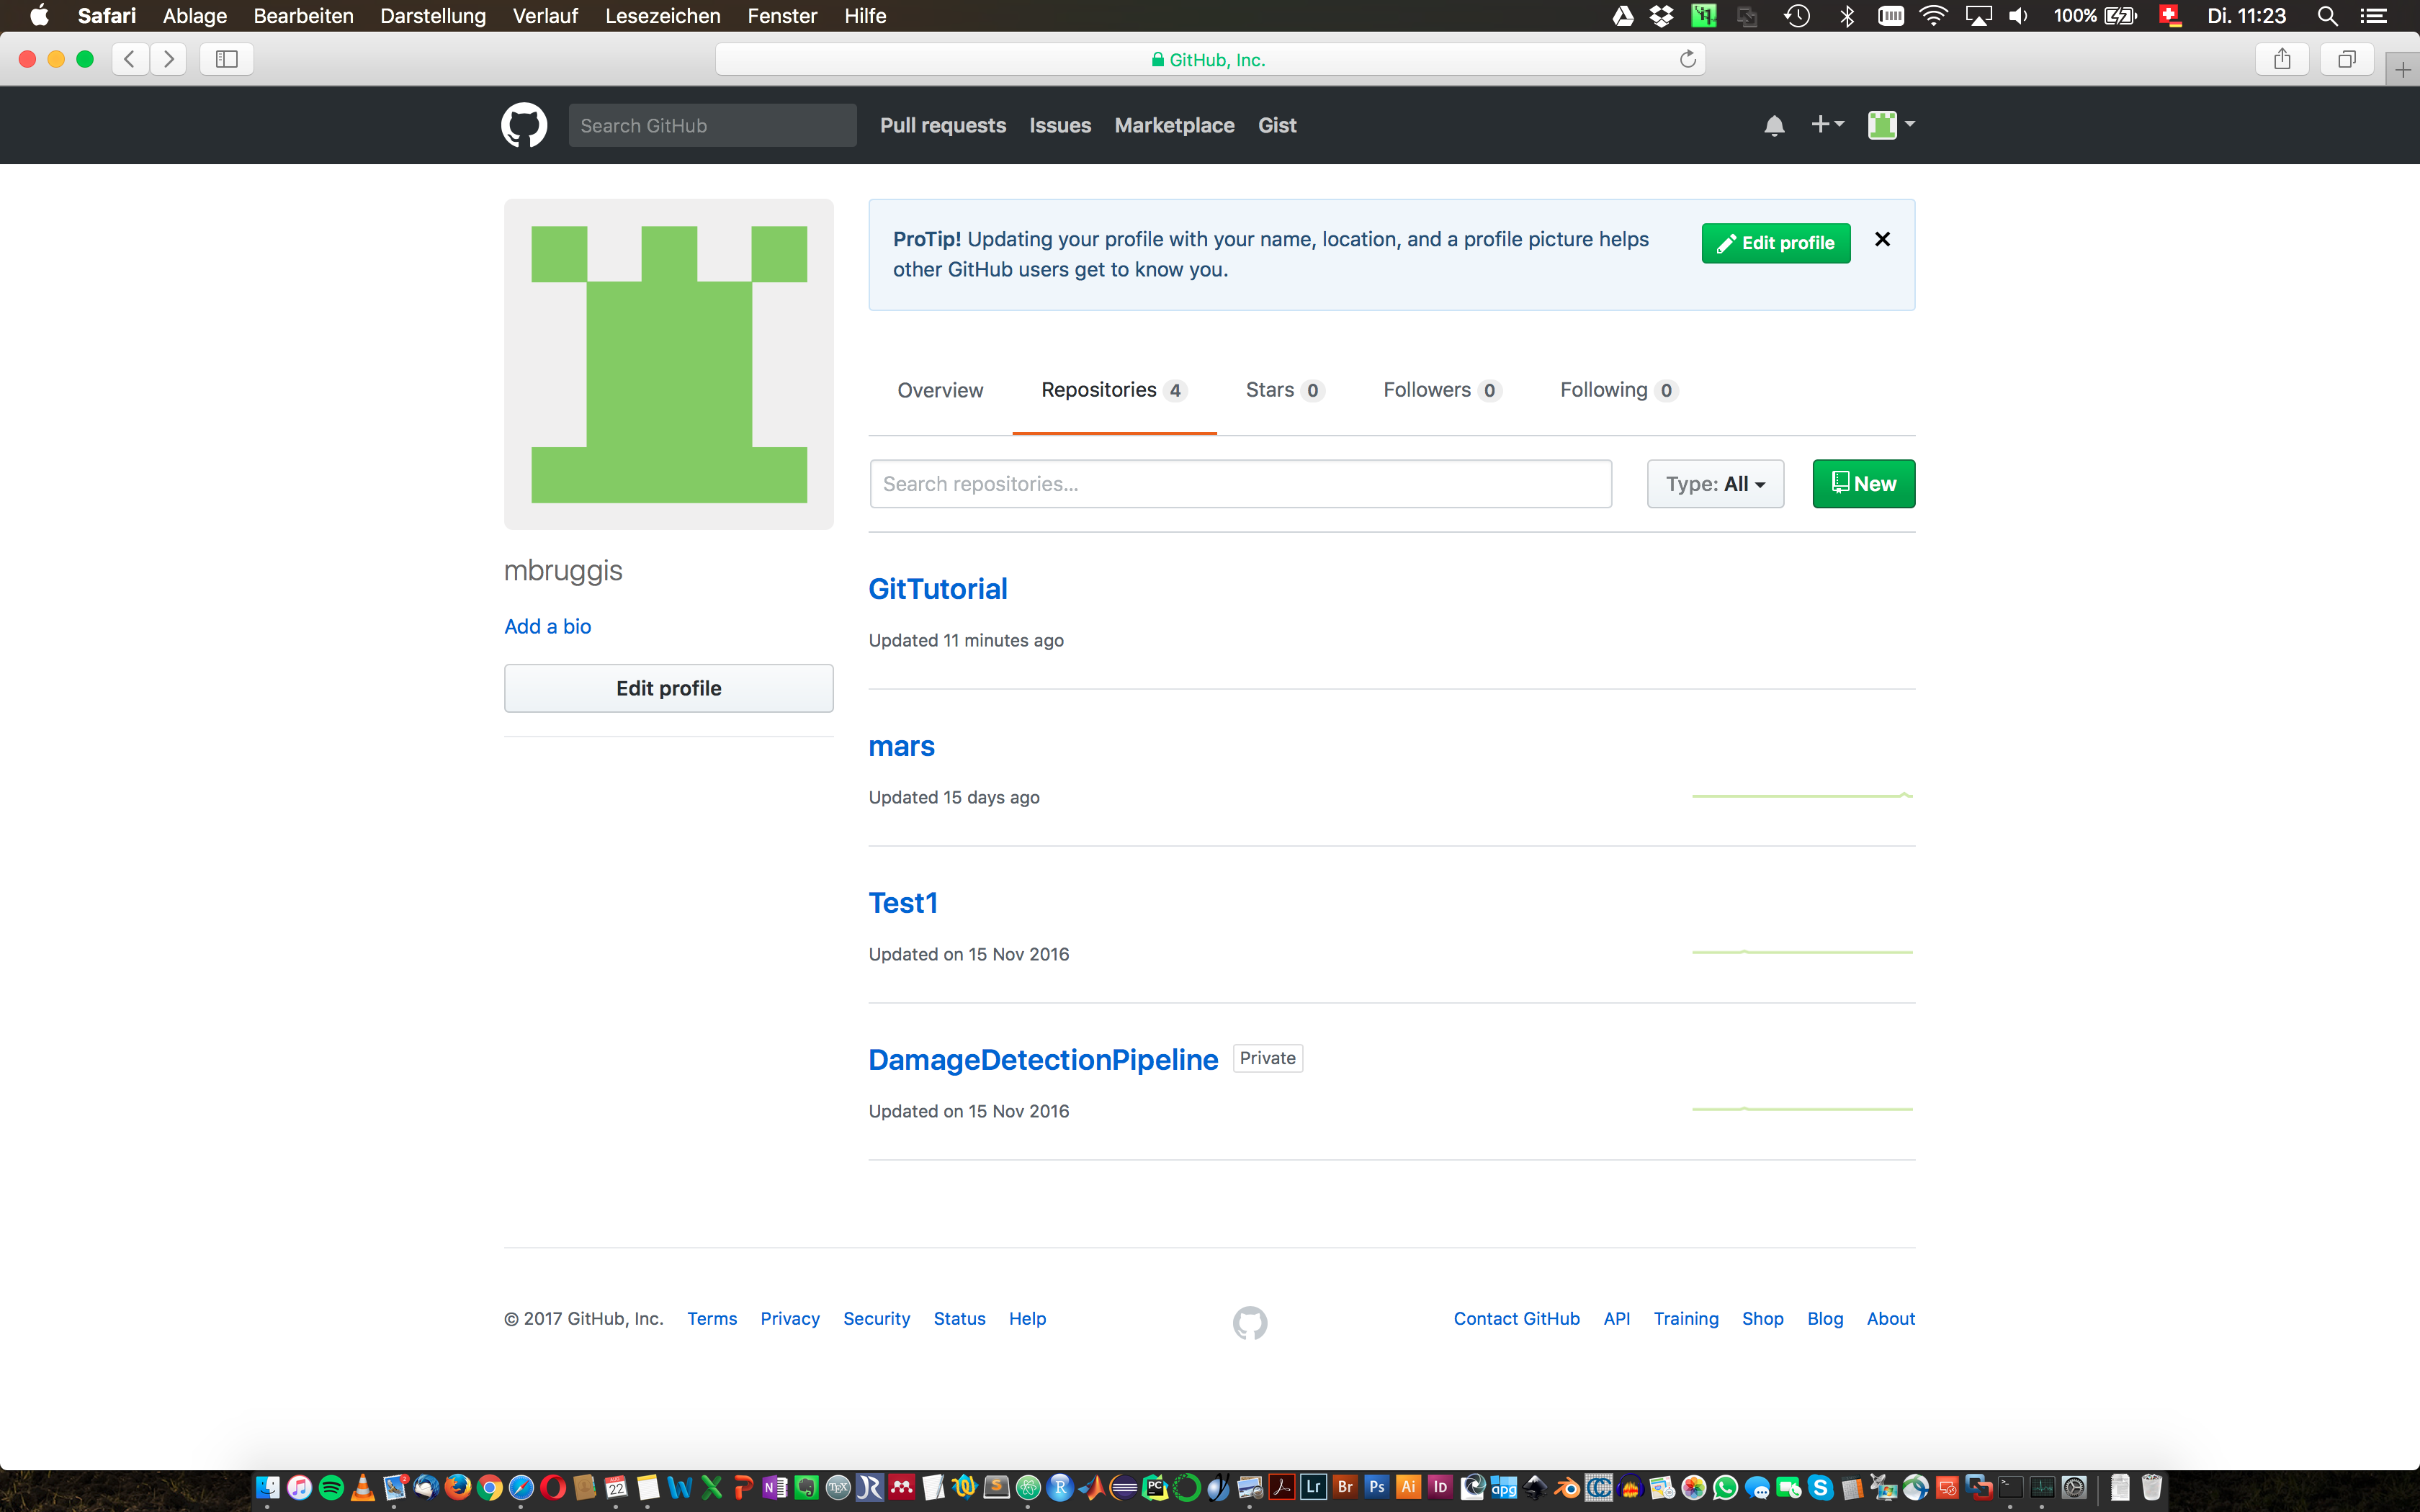
\includegraphics[height=9cm]{./GithubPlatform.png}\label{pc:platform}
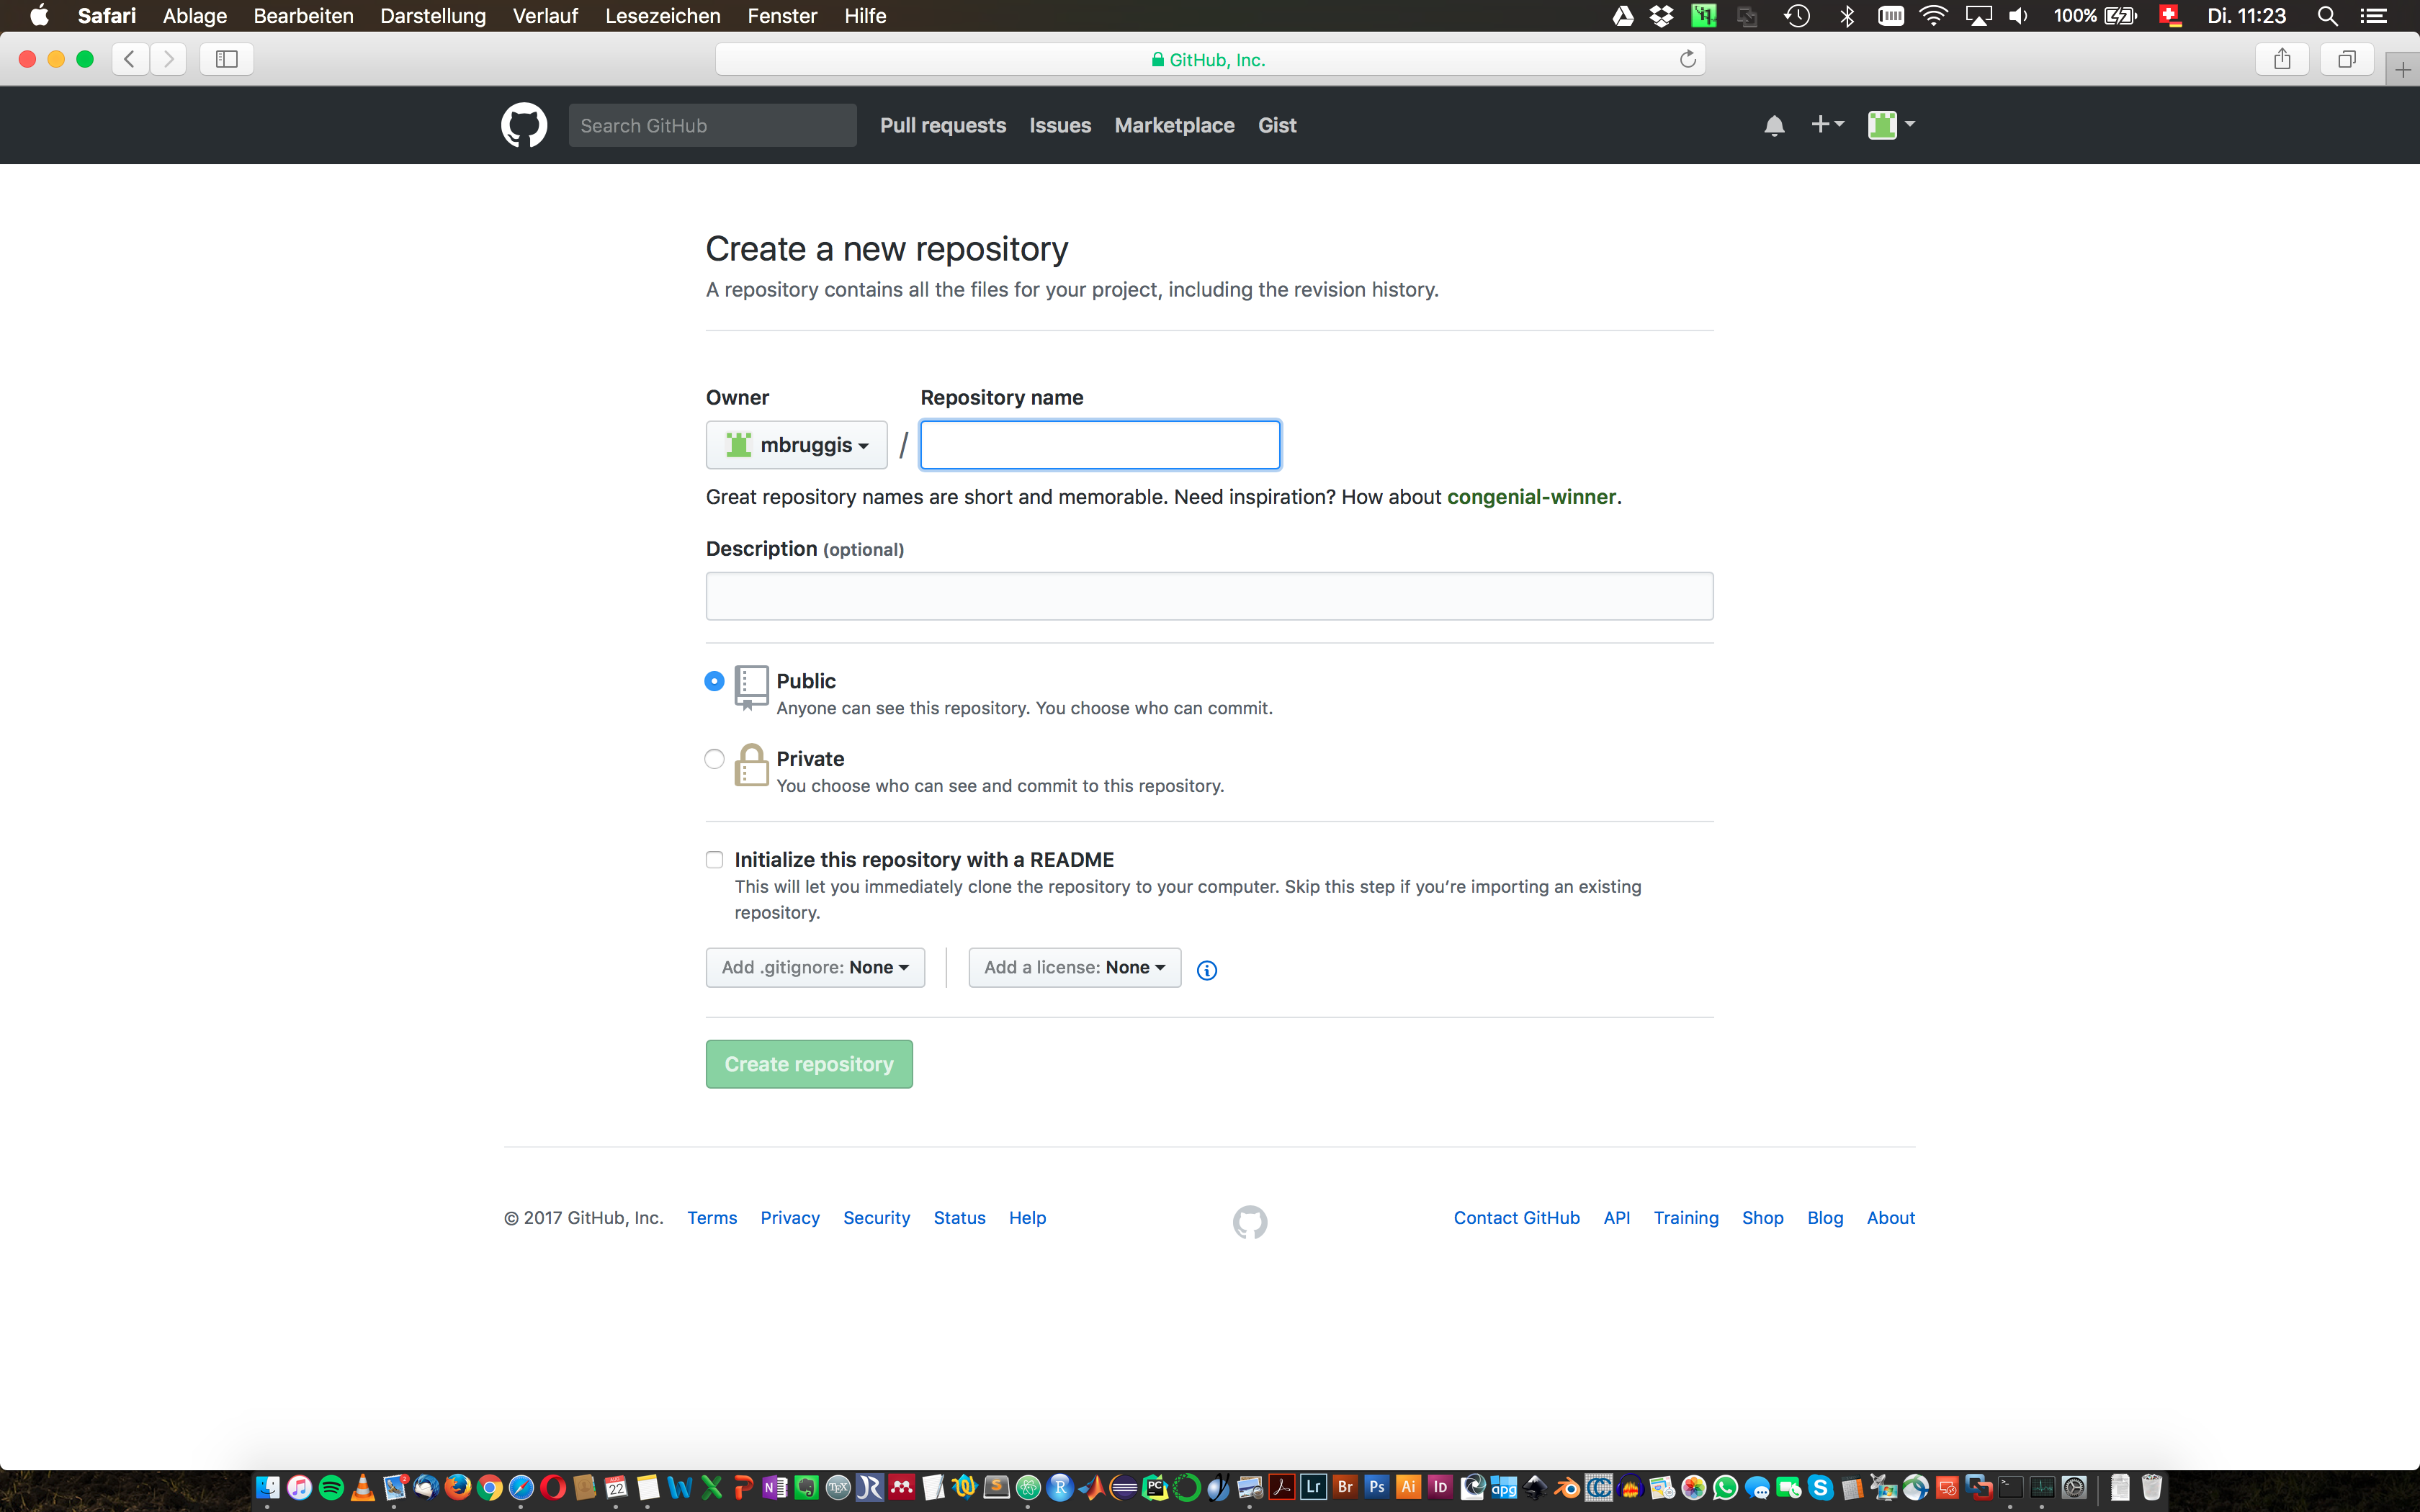
\includegraphics[height=9cm]{./NewRepo.png}\label{pc:overview} \caption[]{Neues Repo wird online auf der Homepage von Github erstellt.}
\label{abb:neuesRepo}
\end{minipage}
}
\end{figure*}

\noindent
In diesem Fall heisst das Repo ganz offensichtlich GitTutorial.

\subsection{Lokalen Ordner erstellen}
Parallel zum Repo auf Github, wird ein lokaler Ordner benötigt, in welchen die zu bearbeitenden Files jeweils gespeichert werden, bevor sie wieder auf den Server hochgeladen werden. Freaks machen dies bekanntlich ja über

\begin{lstlisting}
mkdir path/to/project/project
\end{lstlisting}

\noindent
, wichtig hier ist einfach, dass man übers Terminal in dieses Verzeichnis geht:

\begin{lstlisting}
cd path/to/project/project
\end{lstlisting}

\noindent
Nun kann muss man Git initialisieren, sprich sagen, dass das lokale Repo in diesem Ordner ist:

\begin{lstlisting}
git init
\end{lstlisting}

\noindent
Um zu überprüfen, ob Git nun den richtigen Pfad verwendet, fragt man den Status ab:

\begin{lstlisting}
git status
\end{lstlisting}

\noindent
Da ich hier einen Ordner auf dem Desktop verwende (\textit{Git$\_$Tutorial}), wird mir im Termianal folgende Zeile angegeben:

\begin{lstlisting}
Reinitialized existing Git repository in /Users/Moritz/Desktop/Git_Tutorial/.git/
\end{lstlisting}

\noindent
Hinweis: der \textit{.git}-Ordner, welcher hier ausgegeben wird, ist auf macOS ein versteckter Ordner im Verzeichnis \textit{Git$\_$Tutorial}.

\subsection{File dem \textit{lokalen} Verzeichnis hinzufügen}\label{ch:push}

\subsubsection{\textit{add}-Befehl}

Wenn nun ein File geschrieben wird (alle möglichen Files mit Text sind meines Wissens nach denkbar), wird dieses vorerst lokal im File system gespeichert (vgl. Abbildung \ref{abb:areas}). Um dieses File später dem Git-Verzeichnis hinzu fügen zu können, muss dieses File vorerst in die \textit{staging area} übertragen werden (Abbildung \ref{abb:areas}; im Tutorial, von welchem ich hier viele Infos übernehme, heisst dieses Level \textit{staging area}, keine Ahnung, ob dies ein allgemein gülitger Begriff ist). Folglich werden später nicht alle Files, welche im ursprünglichen Verzeichnis (hier: \textit{Git$\_$Tutorial}) gespeichert sind, im \textit{commit}-Schritt (Kapitel \ref{ch:commit}) ins Git-Verzeichnis übertragen.

\begin{figure*}[!tbph]
\makebox[\textwidth][c]{\begin{minipage}[c]{\textwidth}
\centering
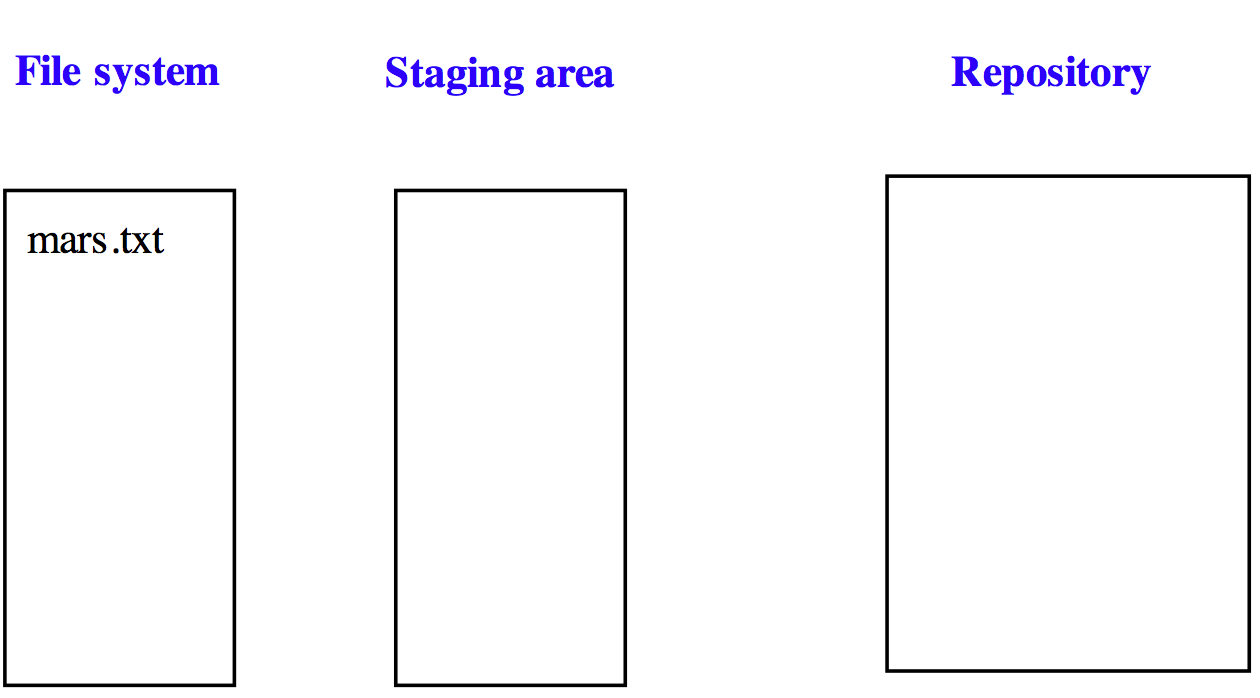
\includegraphics[height=6cm]{./areas.png}
 \caption[]{Überblick über die unterschiedlichen Sphären des File-Systems.}
\label{abb:areas}
\end{minipage}
}
\end{figure*}

\noindent
Files werden über den \textit{add}-Befehl der staging area hinzugefügt (Abbildung \ref{abb:add}):

\begin{lstlisting}
git add FILENAME
\end{lstlisting}

\begin{figure*}[!tbph]
\makebox[\textwidth][c]{\begin{minipage}[c]{\textwidth}
\centering
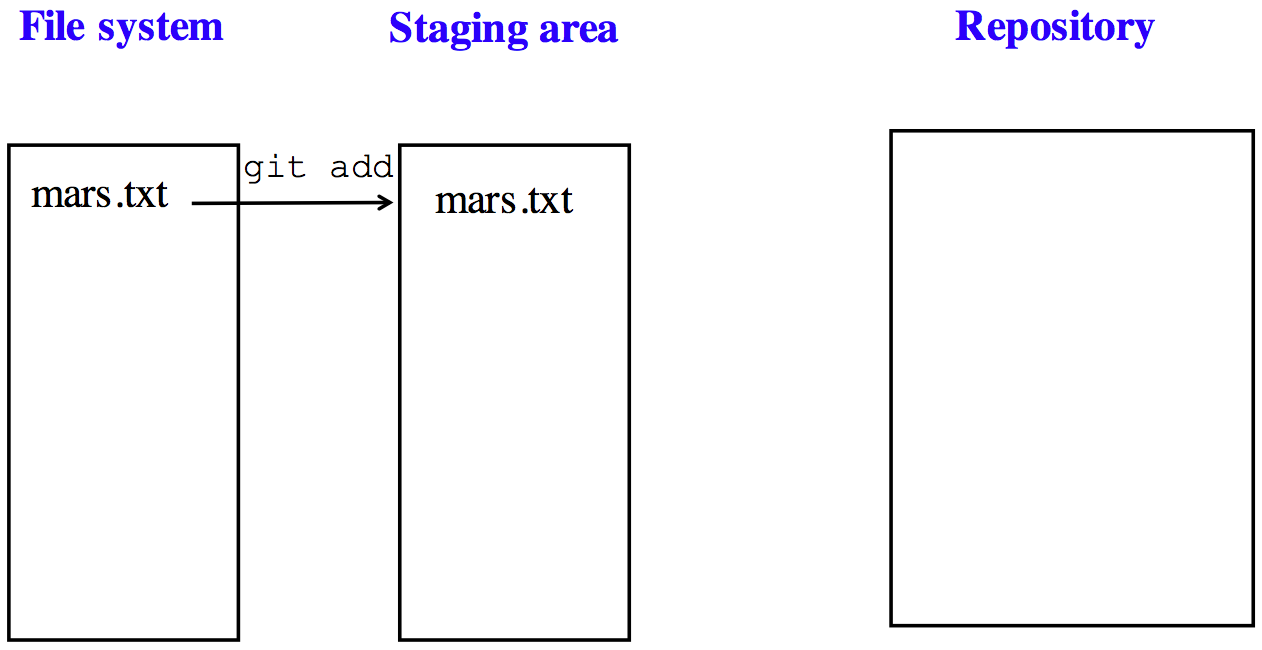
\includegraphics[height=6cm]{./add.png}
 \caption[]{Der add-Befehl fügt ein file der staging-area hinzu.}
\label{abb:add}
\end{minipage}
}
\end{figure*}


\noindent
Über den \textit{status}-Befehl kann überprüft werden, welche Files geadded wurden (Abbildung \ref{abb:statusabfrageadd}).

\begin{figure*}[!tbph]
\makebox[\textwidth][c]{\begin{minipage}[c]{\textwidth}
\centering
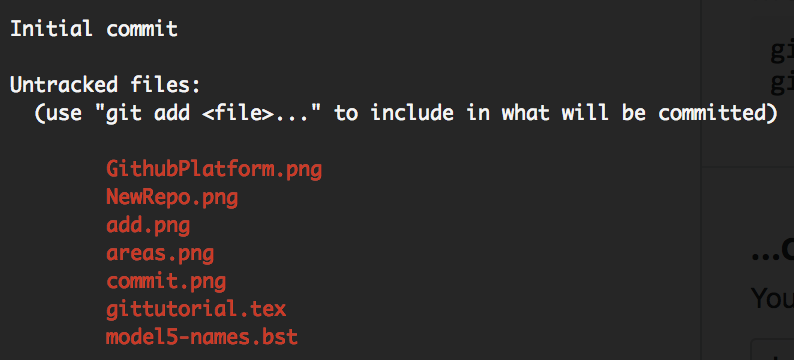
\includegraphics[height=4cm]{./preadd.png}\label{abb:pre}
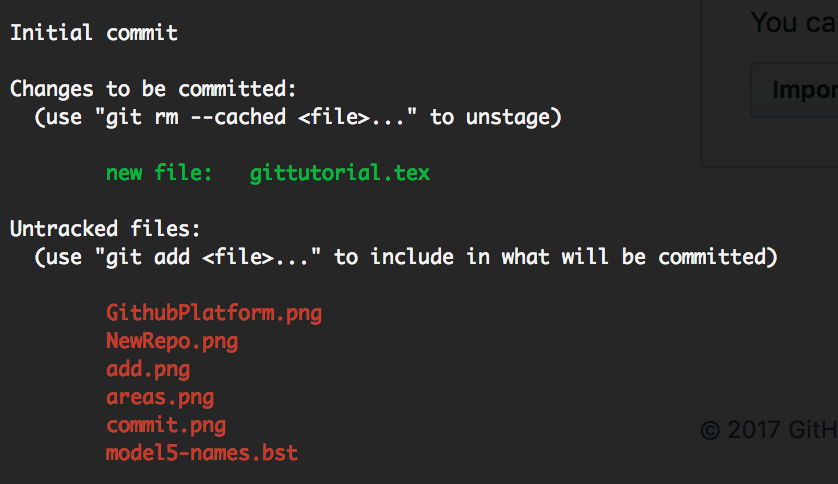
\includegraphics[height=4cm]{./postadd.png}\label{abb:post} \caption[]{Statusinformation über geaddete Files vor (links) und nachdem (rechts) das File gittutorial.tex der staging-area hinzugefügt wurde.}
\label{abb:statusabfrageadd}
\end{minipage}
}
\end{figure*}


\subsubsection{\textit{commit}-Befehl} \label{ch:commit}

Schliesslich muss das File jetzt noch ins Repo committed werden, was über den Befehl \textit{commit} geschieht:

\begin{lstlisting}
git commit -m "message"
\end{lstlisting}

Über diesen Befehl werden die Files in der staging-area nun ins lokale Repo übertragen (Abbildung \ref{abb:commit}). -m \glqq message\grqq wird dabei verwendet, um einen Hinweis zu geben bezüglich der Änderungen, welche vorgenommen wurden gegenüber der Vorversion (und ist glaubs zwingend).\newline
\par
\noindent
Über die Statusabfrage kann nun überprüft werden, welche Files im Repository modifiziert wurden.

\begin{figure*}[!tbph]
\makebox[\textwidth][c]{\begin{minipage}[c]{\textwidth}
\centering
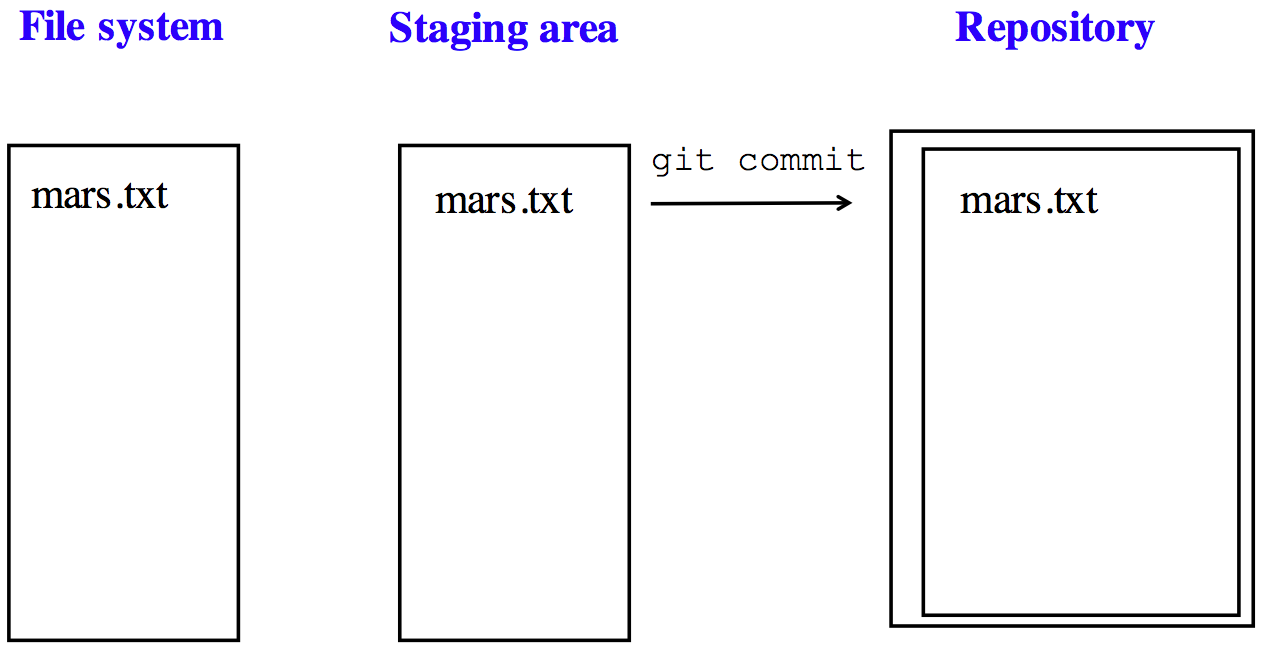
\includegraphics[height=6cm]{./commit.png}
 \caption[]{Der commit-Befehl überträgt die Files in der staging-area ins Repository, welches später mit dem Server synchronisiert wird.}
\label{abb:commit}
\end{minipage}
}
\end{figure*}


\subsubsection{File ändern und Änderungen anzeigen}

Wenn nun ein File im lokalen Ordner (file system) geändert wird, kann man sich die Änderungen gegenüber der Version im Repo anzeigen lassen. Dazu verwendet man den \textit{git diff}-Befehl. Dieser zeigt dann an, welche Zeilen im Text-File abgeändert wurden (Abbildung \ref{abb:diffs}).

\begin{figure*}[!tbph]
\makebox[\textwidth][c]{\begin{minipage}[c]{\textwidth}
\centering
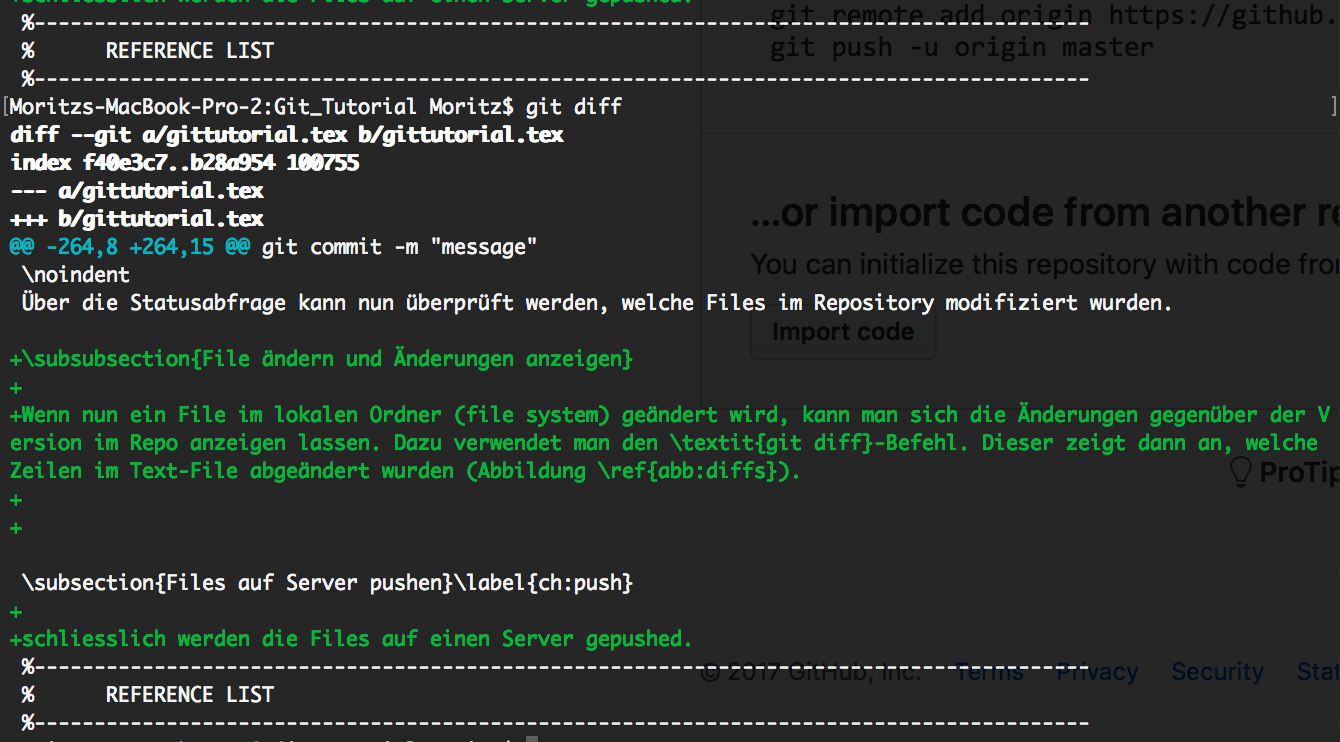
\includegraphics[height=6cm]{./diffs.png}
 \caption[]{Im Terminal wird angezeigt, welche Zeilen im Dokument geändert wurden gegenüber dem File im Repository.}
\label{abb:diffs}
\end{minipage}
}
\end{figure*}

\subsection{Files in Repository auf dem Server übertragen}\label{ch:push}

Im letzten Schritt werden die Files aus dem lokalen Repo ins Repo auf dem Server gepushed. Dazu sind die Informationen erforderlich, welche nach dem Erstellen des Repos auf Github (Kapitel \ref{ch:gitRepo}). angegeben werden (für unser Beispiel in Abbildung \ref{abb:instructions}).

\begin{figure*}[!tbph]
\makebox[\textwidth][c]{\begin{minipage}[c]{\textwidth}
\centering
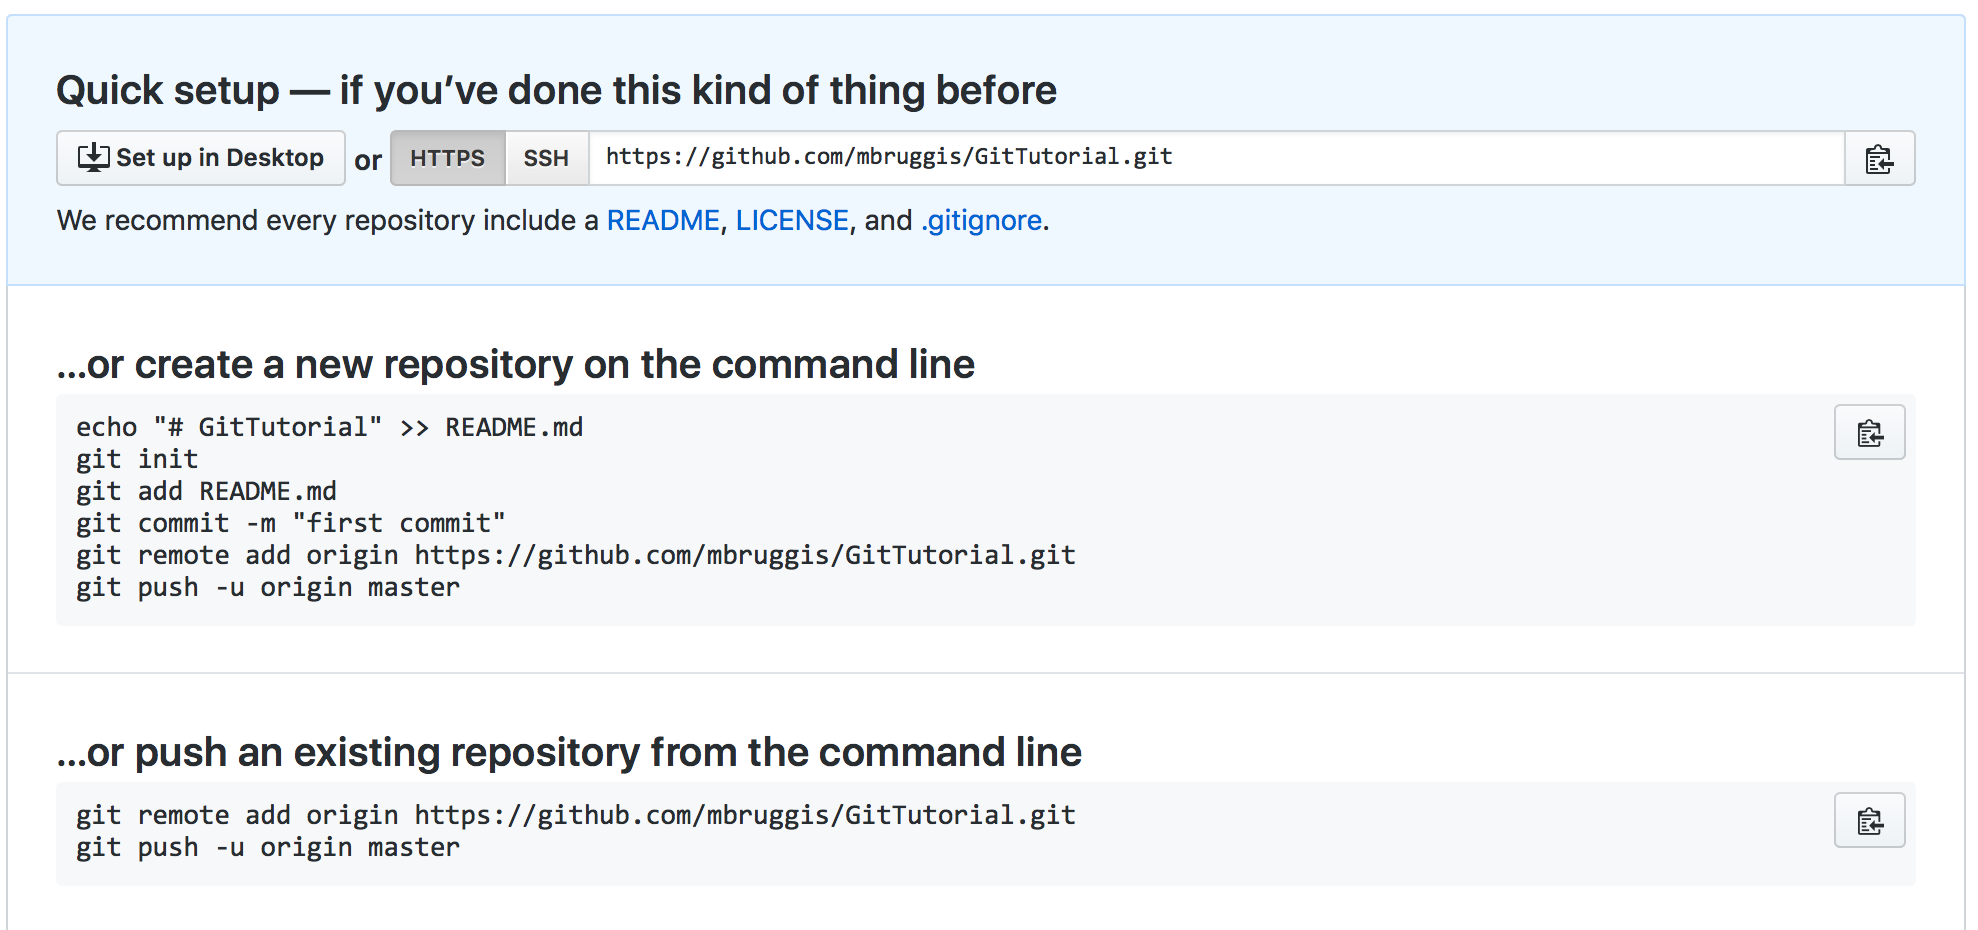
\includegraphics[height=7cm]{./instructions.png}
 \caption[]{Im Terminal wird angezeigt, welche Zeilen im Dokument geändert wurden gegenüber dem File im Repository.}
\label{abb:instructions}
\end{minipage}
}
\end{figure*}

\subsubsection{Lokales Repo mit Repo auf dem Server verknüpfen}

Zuerst müssen das Repo auf dem lokalen Rechner (vgl. Abbildung \ref{abb:areas}) mit demjenigen auf dem Server (erstellt wie in Kapitel \ref{ch:gitRepo} gezeigt) verknüpft werden. Dazu ist der Link notwenig, welcher durch Github angegeben wird (Abbildung \ref{abb:instructions}):

\begin{lstlisting}
git remote add origin https://github.com/mbruggis/GitTutorial.git
\end{lstlisting}

\subsubsection{Files auf Server pushen}
Der letzte Schritt besteht nun darin, die lokal gespeicherten Files auf den Server hochzuladen (vgl. Abbildung \ref{abb:serveroverview}). Dies geschieht über den \textit{push}-Befehl und ist auch bereits in Abbildung \ref{abb:instructions} aufgezeigt:

\begin{lstlisting}
git push -u origin master
\end{lstlisting}

Ich denke mal, master bezeichnet hier den Branch, auf den gepushed wird. Aber hier bin ich noch nicht so bewandert ;-).

\begin{figure*}[!tbph]
\makebox[\textwidth][c]{\begin{minipage}[c]{\textwidth}
\centering
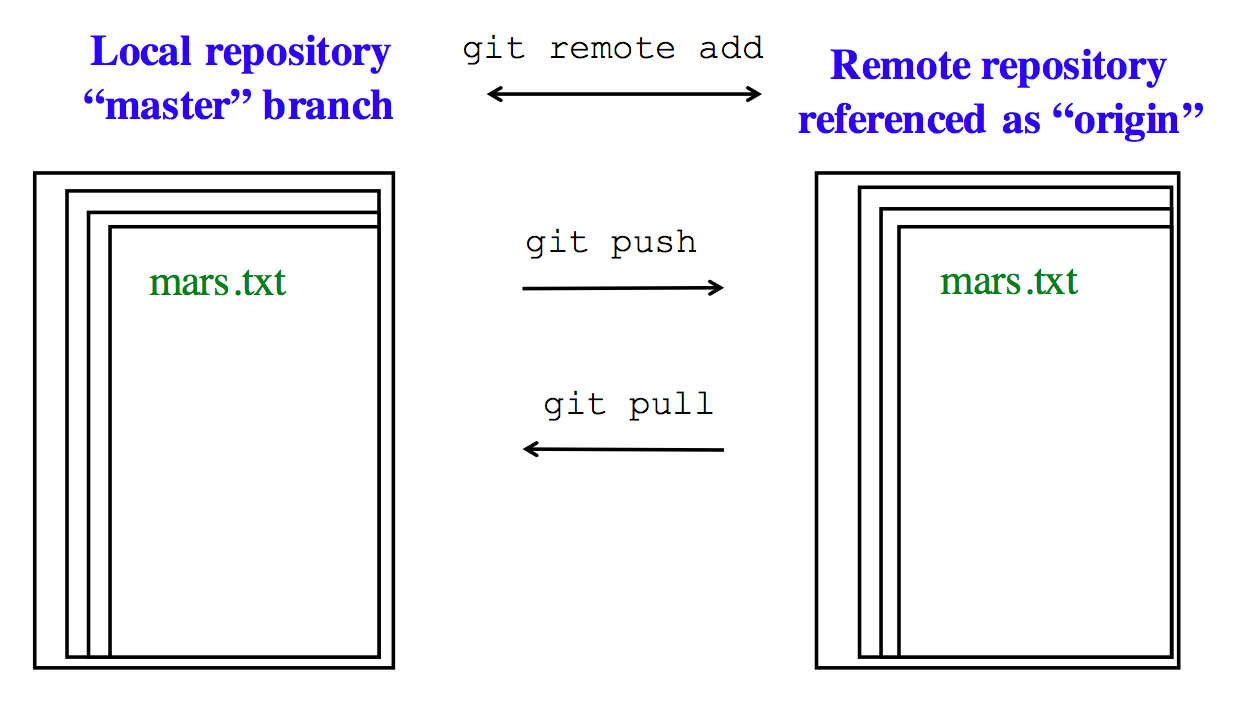
\includegraphics[height=7cm]{./serverOverview.png}
 \caption[]{Überblick über die Befehle, um die Files im lokalen Git-Repo auf den Server hochzuladen und umgekehrt.}
\label{abb:serveroverview}
\end{minipage}
}
\end{figure*}

\subsubsection{Änderungen vom Server übernehmen}

Hat jemand anderes ein File im Repo auf dem Server verändert, muss die aktuelle Version zuerst übernommen werden, um spätere Konflikte zu vermeiden. Dies geschieht über den \textit{pull}-Befehl:

\begin{lstlisting}
git pull
\end{lstlisting}

Allerdings konnte ich dies noch nicht austesten, da ich ja bisher immer nur alleine an den Projekten gearbeitet habe...


\subsection{Weiteres Vorgehen}

Um ein bearbeitetes File wieder hochzuladen, wiederholt man einfach \textit{add} (sehr wichtig, da die Änderungen zuerst in die staging-area übertragen werden müssen! Wird dieser Schritt nicht ausgeführt, weiss Git gar nicht, was verändert wurde am File im lokalen File system), \textit{commit} (um die Änderungen in die staging area zu übernehmen) und \textit{push} (um die Änderungen hochzuladen).\par
Den Verlauf eines Files kann man schliesslich auch auf Github grafisch anschauen, indem man ein File anklickt (öffnet) und sich dann die History anzeigen lässt (Abbildung \ref{abb:history}). Hier erscheinen dann auch (die hier nicht sehr sinnvollen) messages, welche beim committen mitgegeben werden.\par
Der grosse Vorteil hier ist dann, dass man keine alten Versionen mehr verliert, weil man immer Zugriff auf die älteren committeten Versionen hat! Also immer schön committen, Kinder :-).

\begin{figure*}[!tbph]
\makebox[\textwidth][c]{\begin{minipage}[c]{\textwidth}
\centering
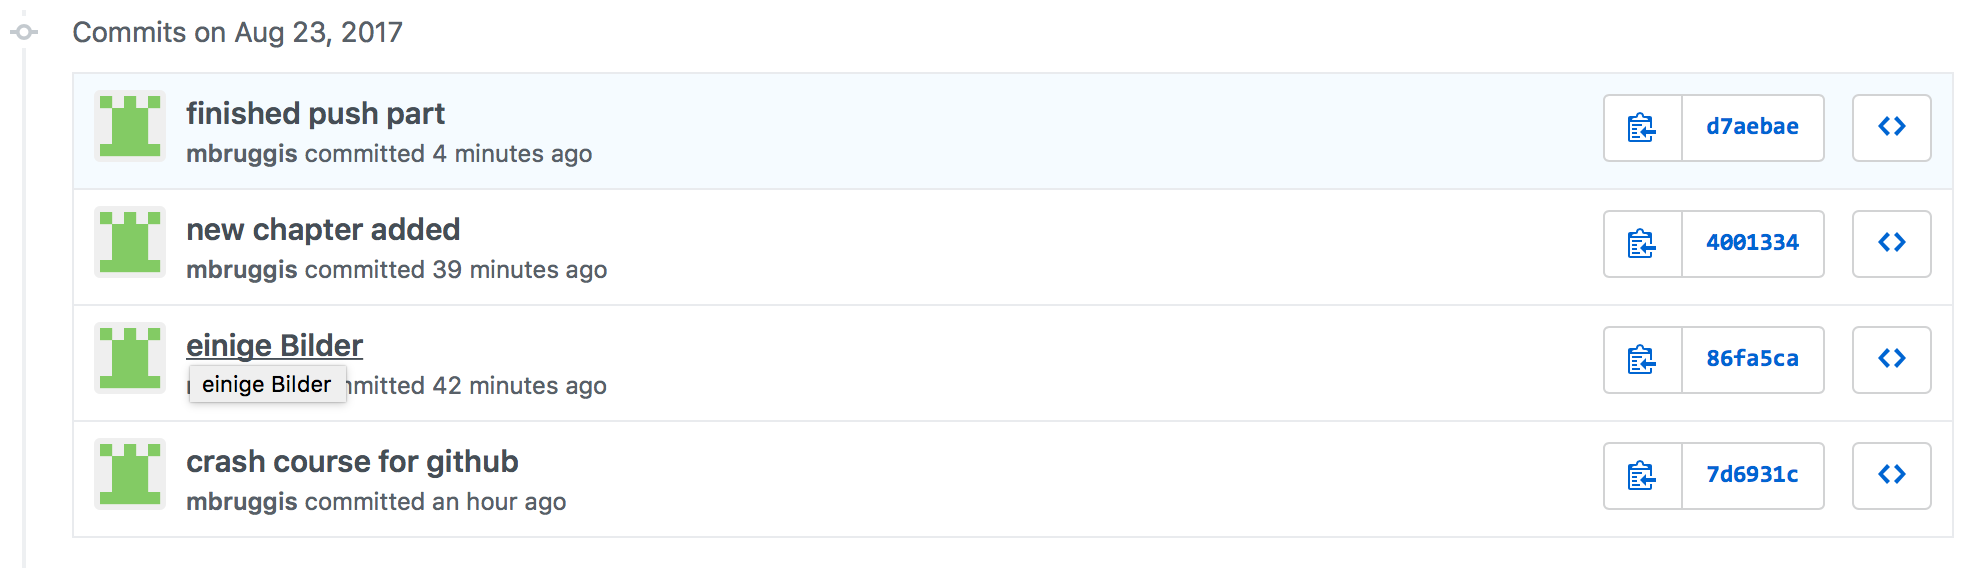
\includegraphics[height=7cm]{./history.png}
 \caption[]{Die unterschiedlichen Versionen eines Files inklusive der Kommentare bezüglich den Veränderungen aus dem commit-Schritt lassen sich anzeigen.}
\label{abb:history}
\end{minipage}
}
\end{figure*}

\subsubsection{Wichtige Überlegungen}

Folgende zwei wichtigen Punkte werden in richtigen Projekten mit mehreren Beteiligten auftreten:

\begin{itemize}
  \item Konflikte
  \item Zusammenführen von Branches
\end{itemize}

Wie das genau läuft, weiss ich jetzt auch nicht. Ihr könnt mein Dokument jedoch gerne weiter bearbeiten :-).

\section{Files von Github herunterladen}

Falls ihr ein Git-Repo von einem Server auf euren Rechner herunterladen wollt, könnt ihr dies einfach tun über den \textit{clone}-Befehl. Ich geb euch mein Repo mal frei, damit ihr das Tutorial ergänzen könnt:

\begin{lstlisting}
git clone https://github.com/mbruggis/GitTutorial.git
\end{lstlisting}

Wichtig ist, dass ihr vor dem Ausführen in das Verzeichnis navigiert, in welches der Ordner heruntergeladen werden soll.


%----------------------------------------------------------------------------------------
%	REFERENCE LIST
%----------------------------------------------------------------------------------------

%\begin{thebibliography}{99} % Bibliography - this is intentionally simple in this template

%\bibliographystyle {physGG6}
%\newpage

%\bibliographystyle{model5-names}
%\bibliography{lit}


%\end{thebibliography}

%----------------------------------------------------------------------------------------

%\end{multicols}

\end{document}
